\documentclass[a4paper]{article}

\addtolength{\hoffset}{-2.25cm}
\addtolength{\textwidth}{4.5cm}
\addtolength{\voffset}{-3.25cm}
\addtolength{\textheight}{5cm}
\setlength{\parskip}{0pt}
\setlength{\parindent}{0in}

%----------------------------------------------------------------------------------------
%	PACKAGES AND OTHER DOCUMENT CONFIGURATIONS
%----------------------------------------------------------------------------------------

\usepackage{blindtext} % Package to generate dummy text
\usepackage{charter} % Use the Charter font
\usepackage[utf8]{inputenc} % Use UTF-8 encoding
\usepackage{microtype} % Slightly tweak font spacing for aesthetics
\usepackage[english]{babel} % Language hyphenation and typographical rules
\usepackage{amsthm, amsmath, amssymb} % Mathematical typesetting
\usepackage{float} % Improved interface for floating objects
\usepackage[final, colorlinks = true,
            linkcolor = black,
            citecolor = black]{hyperref} % For hyperlinks in the PDF
\usepackage{graphicx, multicol} % Enhanced support for graphics
\usepackage{xcolor} % Driver-independent color extensions
\usepackage{marvosym, wasysym} % More symbols
\usepackage{rotating} % Rotation tools
\usepackage{censor} % Facilities for controlling restricted text
\usepackage{listings} % Environment for non-formatted code, !uses style file!
\usepackage{pseudocode} % Environment for specifying algorithms in a natural way
 % Environment for f-structures, !uses style file!
\usepackage{booktabs} % Enhances quality of tables
\usepackage{tikz-qtree} % Easy tree drawing tool
 % Configuration for b-trees and b+-trees, !uses style file!
\usepackage[backend=biber,style=numeric,
            sorting=nyt]{biblatex} % Complete reimplementation of bibliographic facilities
\addbibresource{ecl.bib}
\usepackage{csquotes} % Context sensitive quotation facilities
\usepackage[yyyymmdd]{datetime} % Uses YEAR-MONTH-DAY format for dates
\renewcommand{\dateseparator}{-} % Sets dateseparator to '-'
\usepackage{fancyhdr} % Headers and footers
\pagestyle{fancy} % All pages have headers and footers
\fancyhead{}\renewcommand{\headrulewidth}{0pt} % Blank out the default header
\fancyfoot[L]{} % Custom footer text
\fancyfoot[C]{} % Custom footer text
\fancyfoot[R]{\thepage} % Custom footer text
\newcommand{\note}[1]{\marginpar{\scriptsize \textcolor{red}{#1}}} % Enables comments in red on margin
\usepackage{mathtools}
\usepackage{amsmath}
\DeclarePairedDelimiter\abs{\lvert}{\rvert}%
\usepackage{cancel}
\usepackage{minted}
\usepackage{float}
\usepackage{caption}
\usepackage{subcaption}
%-------------------------------

%----------------------------------------------------------------------------------------

%-------------------------------
%	ENVIRONMENT SECTION
%-------------------------------
\pagestyle{fancy}
\usepackage{mdframed}

\usepackage[sfdefault]{FiraSans} %% option 'sfdefault' activates Fira Sans as the default text font
\usepackage[T1]{fontenc}
\renewcommand*\oldstylenums[1]{{\firaoldstyle #1}}


% remove numbering from sections
\usepackage{titlesec}
\titleformat{\section}{\normalfont\Large\bfseries}{}{0pt}{}



%-------------------------------------------------------------------------------------------
%	CUSTOM COMMANDS
%-------------------------------
\newcommand{\gaussian}{\frac{1}{\sigma\sqrt{2\pi}}\exp\left(- \frac{(x-\mu)^2}{2\sigma^2}\right)}
\newcommand{\R}{\mathbb R}

\def\inline{\lstinline[basicstyle=\ttfamily,keywordstyle={}]}


\begin{document}


%-------------------------------
%	TITLE SECTION
%-------------------------------

\fancyhead[C]{}
\hrule \medskip % Upper rule
\begin{minipage}{0.295\textwidth}
\raggedright
\footnotesize
Francisco Javier Sáez Maldonado \hfill\\
franciscojavier.saez@estudiante.uam.es
\hfill\\
\end{minipage}
\begin{minipage}{0.4\textwidth}
\centering
\large
Fingerprint Lab Report\\
\normalsize
Deep Learning for Biometric Signal Processing\\
\end{minipage}
\begin{minipage}{0.295\textwidth}
\raggedleft
\today\hfill\\
\end{minipage}
\medskip\hrule

%-------------------------------
%	CONTENTS
%-------------------------------
\section{Exercise 1}
\subsection{ Copy here the two fingerprint images provided as examples example1\_1 and example1\_2}

We are provided with the following to examples of fingerprints.

\begin{figure}[H]
  \centering
       \begin{subfigure}[t]{0.45\textwidth}
         \centering
         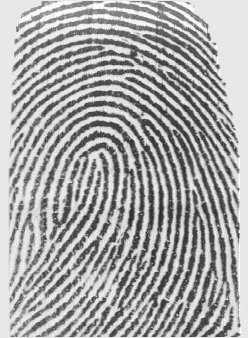
\includegraphics[scale=0.6]{Figures/example1_1}
         \caption{Example1\_1}
     \end{subfigure}%
     \quad
     \begin{subfigure}[t]{0.45\textwidth}
         \centering
         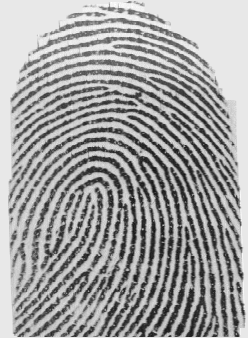
\includegraphics[scale=0.6]{Figures/example1_2}
         \caption{Example1\_2}
     \end{subfigure}
    \caption{Examples of fingerprints.}
    \label{fig:ex1a}
\end{figure}

As we can see, the pictures of the fingerprints have relatively high quality and its macro-singularities can be observed at first sight.

\subsection{ How many macro-singularities do you observe in each fingerprint?}

As we already know, macro-singularities can be loops, deltas or whorls.\\

In the previous figure we can observe a single loop in each of the fingerprints. No deltas or whorls have been found.

\subsection{ Mark the macro-singularities in the images (deltas and loops).}

We mark the previously mentioned loops using a red circle in Figure \ref{fig:ex1b}.

\begin{figure}[H]
  \centering
       \begin{subfigure}[t]{0.45\textwidth}
         \centering
         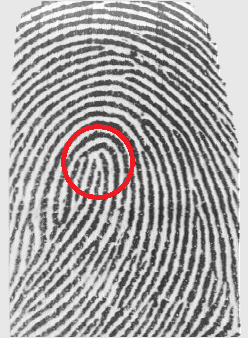
\includegraphics[scale=0.6]{Figures/example1_marked}
         \caption{Example1\_1 with a marked loop.}
     \end{subfigure}%
     \quad
     \begin{subfigure}[t]{0.45\textwidth}
         \centering
         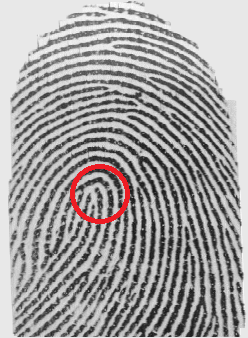
\includegraphics[scale=0.6]{Figures/example2_marked}
         \caption{Example1\_2 with a marked loop.}
     \end{subfigure}
    \caption{Marked loops.}
    \label{fig:ex1b}
\end{figure}

\section{Exercise 2}
\subsection{ Execute the provided code for Fingerprint Enhancement and paste the resulting image here}

We execute the Matlab script \inline{main.m} and stop it when the enhanced images are printed. The obtained enhanced fingerprints are shown in Figure \ref{fig:ex2a}.



\begin{figure}[H]
  \centering
       \begin{subfigure}[t]{0.45\textwidth}
         \centering
         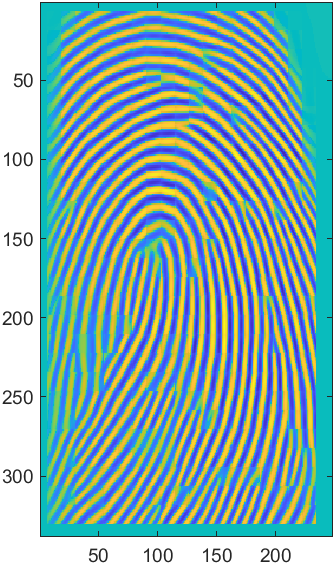
\includegraphics[scale=0.6]{Figures/Enhanced1}
         \caption{Example1\_1 enhanced.}
     \end{subfigure}%
     \quad
     \begin{subfigure}[t]{0.45\textwidth}
         \centering
         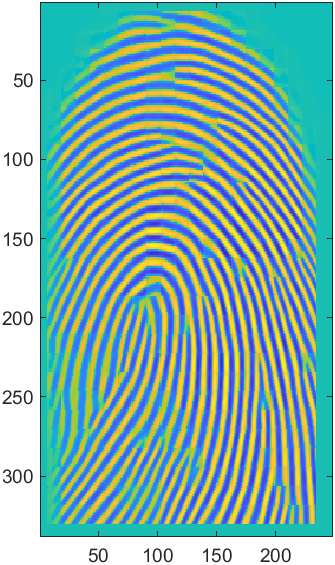
\includegraphics[scale=0.6]{Figures/Enhanced2}
         \caption{Example1\_2 enhanced.}
     \end{subfigure}
    \caption{Enhanced fingerprint examples.}
    \label{fig:ex2a}
\end{figure}


\subsection{ What differences do you observe with respect to the original fingerprints?}

The aim of the enhancement techniques is to improve the fingerprint image quality in order make the feature extraction task easier. Typically, we want to complete the ridge lines, deal with cuts or bruises on the finger or obtain a better separation between parallel ridges.\\

As we can see, the fingerprints in Figure \ref{fig:ex1a} had incomplete ridge lines at the bottom part of the image which have been completed in the enhancement in Figure \ref{fig:ex2a}.\\

Also, the image has been \emph{sharpened}, which means that now the contrast between the ridge lines and the \emph{white spaces} has been increased, making ridge lines easier to identify.


\section{Exercise 3}
\subsection{ Execute now the code for Quality Maps, and paste the resulting quality maps}

If we keep executing the \inline{main.m} script we obtain the following Quality Maps:



\begin{figure}[H]
  \centering
       \begin{subfigure}[t]{0.45\textwidth}
         \centering
         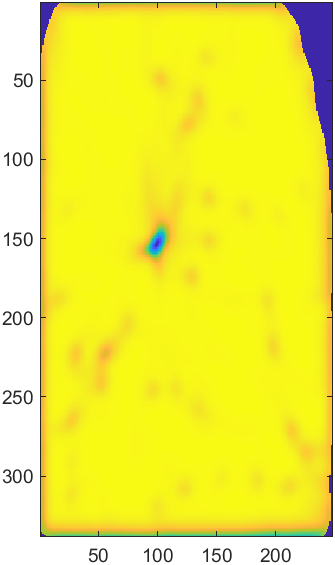
\includegraphics[scale=0.6]{Figures/QMap1}
         \caption{Quality Map of the first fingerprint.}
     \end{subfigure}%
     \quad
     \begin{subfigure}[t]{0.45\textwidth}
         \centering
         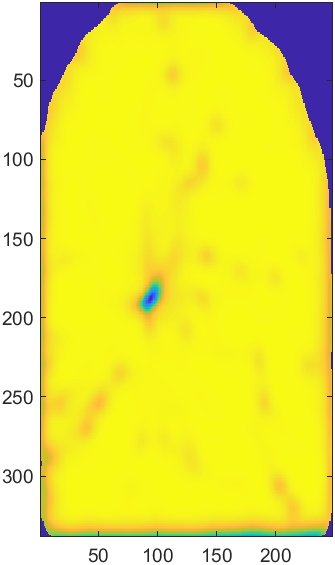
\includegraphics[scale=0.6]{Figures/QMap2}
         \caption{Quality Map of the second fingerprint.}
     \end{subfigure}
    \caption{Quality maps.}
    \label{fig:ex3a}
\end{figure}


\subsection{ What is the range of values for these quality maps?}

To obtain this quantities, we have added the following code to the main script: 

\begin{minted}{Matlab}
  min(relI1,[],'all')
  max(relI1,[],'all')
  
  min(relI2,[],'all')
  max(relI2,[],'all')
\end{minted}

This code shows that:

\begin{itemize}
  \item The minimum value for both Quality Maps is \(0.0\)
  \item The maximum value for the first fingerprint Quality Map is \(0.9991\)
  \item The maximum value for the second fingerprint Quality Map is \(0.9988\)
\end{itemize}

Thus, we can say that both Quality Maps have all its values in the range \([0,1]\).

\subsection{ What kind information (apart from the quality) can be inferred from such code?}

We examine the file \inline{testfin.m} to understand the result that we are obtaining. If we read the first commented lines, we find that the function we applied returns
\begin{minted}{MatLab}
  % Returns:    newim - Ridge enhanced image.
  %             binim - Binary version of enhanced image.
  %             mask  - Ridge-like regions of the image
  %             reliability - 'Reliability' of orientation data  
\end{minted}
Considering this and the code of the \inline{main.m} file, what we just showed in Figure \ref{fig:ex3a} is the \textbf{reliabiltiy} of the orientation data, that is, how secure we are of the orientation of the ridge-lines in each point of the image.\\

As we can see in the figure \ref{fig:ex3a}, we can say that we can not rely on the results \emph{outside} the fingerprint (with outside meaning the white part with no ridge-lines), and that the algorithm has some problems in the zone where the loop is detected. This makes sense to us, since in the top of the loop the orientation of the ridge-line changes completely.\\  

We also find that the process followed to obtain the quality maps is:
\begin{enumerate}
\item Identify the ridge-like regions and normalise the image. We can see that different blocksizes and thresholds have been used but finally using \(blocksize=16\) and \(threshold = 0.1\) are the values used.
\item Determine the orientations of the found ridge-like regions.
\item Determine ridge frequency values across the image. Then, the median frequency is multiplied in the final mask that will be applied to the image (a comment says that the median frequency performed better than the actual frequency).
\item Lastly, the filter is applied to enhance the patterns
\end{enumerate}




\section{Exercise 4}

\subsection{ Execute the code in order to show the Binarized Fingerprint and the Segmented Fingerprint. Apply different values of quality threshold (0.1, 0.3, 0.6, 0.9) and paste here the resulting images}

Let us first examine the code to see what we are doing in this section.

\begin{minted}{MatLab}
  %Binarized and Segmented Fingerprints
  threshold=0.1; %quality threshold
  figure;
  subplot(121)
  imagesc(binI1+mask1+(relI1>threshold)) 
  binI1(relI1<threshold)=0; 
  inv_binI1 = (binI1 == 0); 
\end{minted}

We can see that we stablish a threshold (which we are told to modify) and then plots an image that is an addition of the images:
\begin{itemize}
\item Enhanced binarized image
\item The mask that contains the ridge-like regions of the image (returned by \inline{testfin})
\item The reliability of the orientation, selecting the pixels where the reliability is above the selected threshold
\end{itemize}

The result of the code is shown in Figures \ref{fig:ex4-1st} and \ref{fig:ex4-2nd}.

\begin{figure}[H]
  \centering
       \begin{subfigure}[t]{0.2\textwidth}
         \centering
         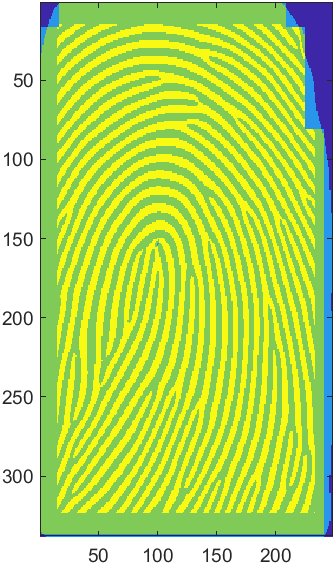
\includegraphics[scale=0.5]{Figures/E4-e1-0.1}
         \caption{\(0.1\)}
     \end{subfigure}%
     \quad
     \begin{subfigure}[t]{0.2\textwidth}
         \centering
         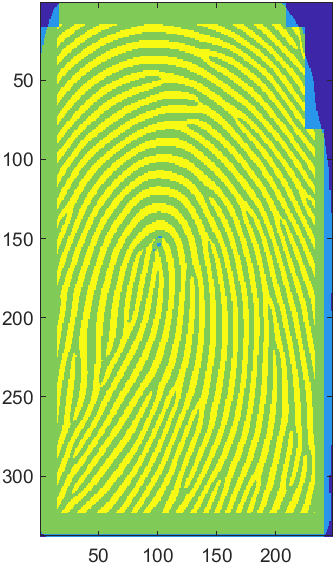
\includegraphics[scale=0.5]{Figures/E4-e1-0.3}
         \caption{\(0.3\)}
     \end{subfigure}
     \begin{subfigure}[t]{0.2\textwidth}
      \centering
      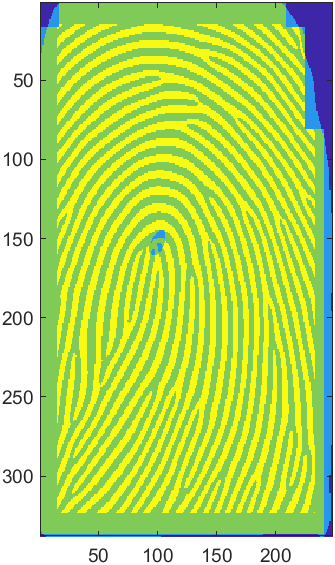
\includegraphics[scale=0.5]{Figures/E4-e1-0.6}
      \caption{\(0.6\)}
  \end{subfigure}%
  \quad
  \begin{subfigure}[t]{0.2\textwidth}
      \centering
      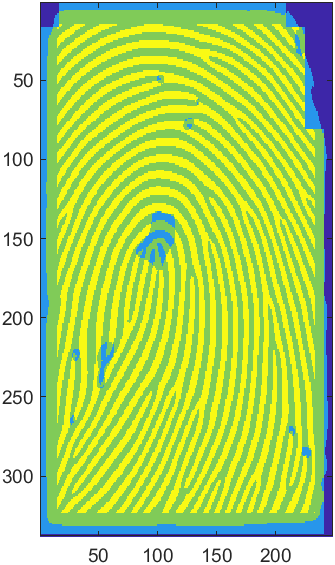
\includegraphics[scale=0.5]{Figures/E4-e1-0.9}
      \caption{\(0.9\)}
  \end{subfigure}
    \caption{Different thresholds for the first fingerprint example.}
    \label{fig:ex4-1st}
\end{figure}

\begin{figure}[H]
  \centering
       \begin{subfigure}[t]{0.2\textwidth}
         \centering
         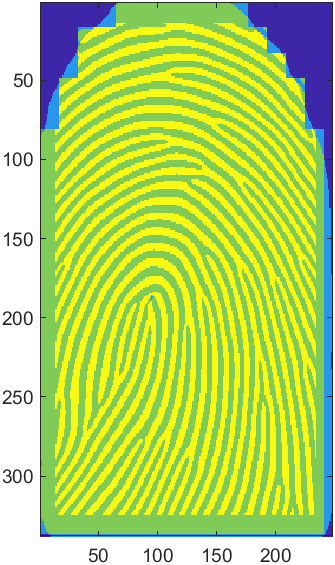
\includegraphics[scale=0.5]{Figures/E4-e2-0.1}
         \caption{\(0.1\)}
     \end{subfigure}%
     \quad
     \begin{subfigure}[t]{0.2\textwidth}
         \centering
         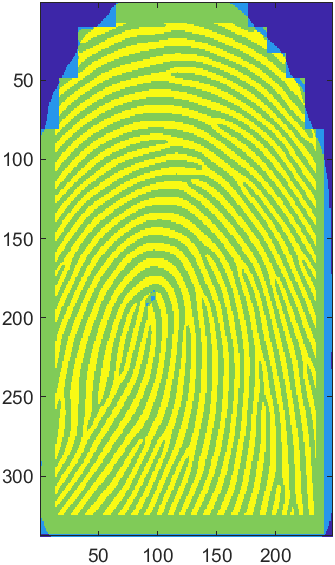
\includegraphics[scale=0.5]{Figures/E4-e2-0.3}
         \caption{\(0.3\)}
     \end{subfigure}
     \begin{subfigure}[t]{0.2\textwidth}
      \centering
      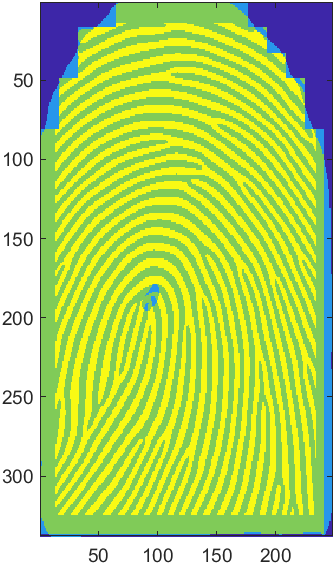
\includegraphics[scale=0.5]{Figures/E4-e2-0.6}
      \caption{\(0.6\)}
  \end{subfigure}%
  \quad
  \begin{subfigure}[t]{0.2\textwidth}
      \centering
      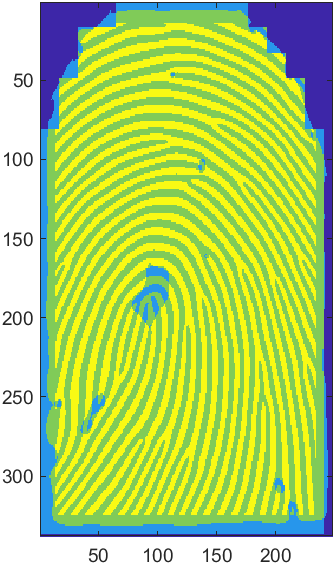
\includegraphics[scale=0.5]{Figures/E4-e2-0.9}
      \caption{\(0.9\)}
  \end{subfigure}
    \caption{Different thresholds for the second fingerprint example.}
    \label{fig:ex4-2nd}
\end{figure}

We can observe in both cases that, as the threshold is increased, the reliability around the loops decreases and the yellow mask dissapear in both cases. This phenomenon also happens in other points that, until this point of the lab, we have not detected as important points.




\section{Exercise 5}
\subsection{ Execute the code for generating the Fingerprint Skeleton and the Minutiae Extractor. Paste the resulting images for the original values \(window=5\) and \(margin=5\). }

Firstly, we show in Figure \ref{fig:ex5a} the skeletons obtained by the function \inline{bwmorph}.

\begin{figure}[H]
  \centering
       \begin{subfigure}[t]{0.45\textwidth}
         \centering
         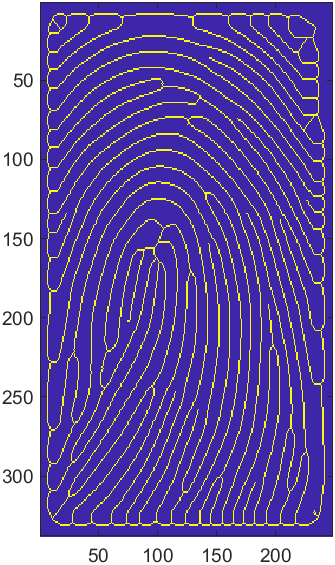
\includegraphics[scale=0.6]{Figures/Skeleton1}
         \caption{Example1\_1}
     \end{subfigure}%
     \quad
     \begin{subfigure}[t]{0.45\textwidth}
         \centering
         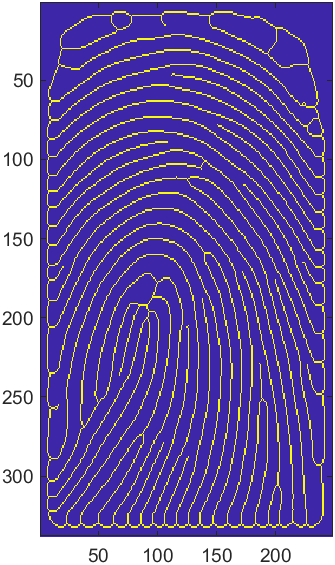
\includegraphics[scale=0.6]{Figures/Skeleton2}
         \caption{Example1\_2}
     \end{subfigure}
    \caption{Skeletons of fingerprints.}
    \label{fig:ex5a}
\end{figure}

We can observe that the fingerprint has been transformed in order to make its shape a bit more \emph{squared} and we have only kept a think line for each ridge-line that we had in the beggining.\\

We now show in Figure \ref{fig:ex5a2} the minutias extracted for each of the skeletons, with the default parameters \(window=5\) and \(margin=5\).

\begin{figure}[H]
  \centering
       \begin{subfigure}[t]{0.45\textwidth}
         \centering
         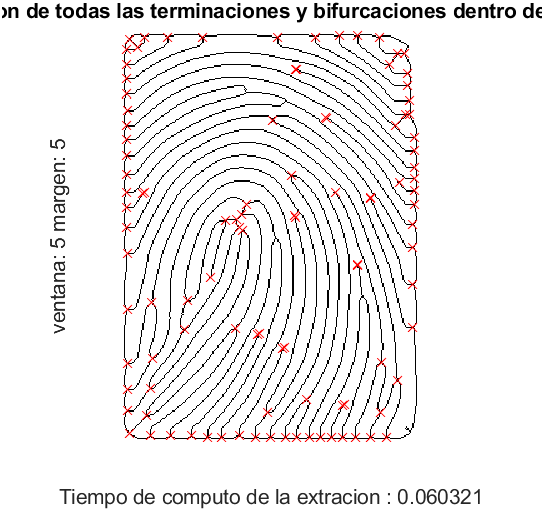
\includegraphics[scale=0.6]{Figures/Minutiae1}
         \caption{Example1\_1}
     \end{subfigure}%
     \quad
     \begin{subfigure}[t]{0.45\textwidth}
         \centering
         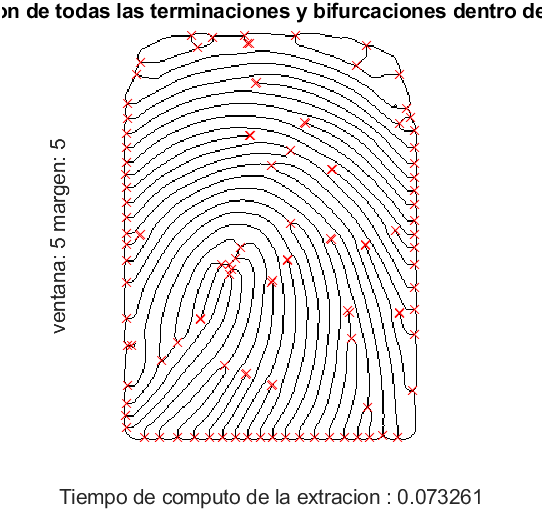
\includegraphics[scale=0.6]{Figures/Minutiae2}
         \caption{Example1\_2}
     \end{subfigure}
    \caption{Minutiae of example fingerprints.}
    \label{fig:ex5a2}
\end{figure}

As we can see, many \emph{minutias} have been found at the edges of the skeleton.


\subsection{Search heuristically by looking at the images for the optimal values of parameters window and margin. Paste the resulting images with your optimal parameters and justify your decision.}

Ideally, we would like to obtain parameters \(window,margin\) such that:
\begin{enumerate}
\item There are not many (or none at all) minutias in the edge of the skeleton.
\item All the minutias are found inside the skeleton, not skipping any of them.
\end{enumerate}

As we have mentioned,in the previous case we found many minutias at the edges, so initially we would like to \textbf{increase the margin}. Also, if we observe the images in Figure \ref{fig:ex5a2}, many minutias have been ignored inside the edges of the skeleton, due to the big window size, so we will \textbf{decrease the window size}.

Firstly, we increase the margin to \(margin = 10\), to check how the minutiae extraction works. We can see the result in Figure \ref{fig:ex5b}

\begin{figure}[H]
  \centering
       \begin{subfigure}[t]{0.45\textwidth}
         \centering
         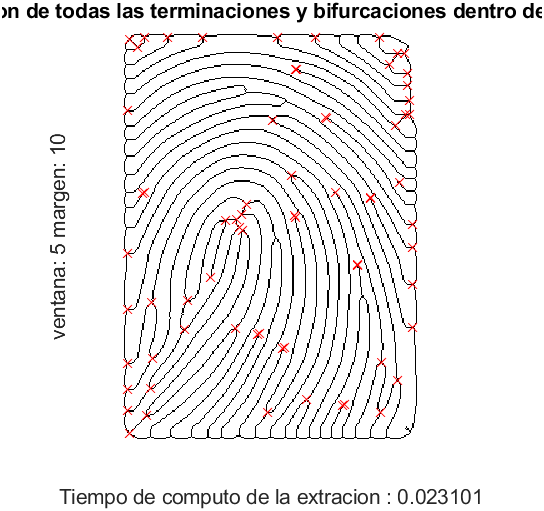
\includegraphics[scale=0.7]{Figures/Minutiae1-m10}
         \caption{Example1\_1}
     \end{subfigure}%
     \quad
     \begin{subfigure}[t]{0.45\textwidth}
         \centering
         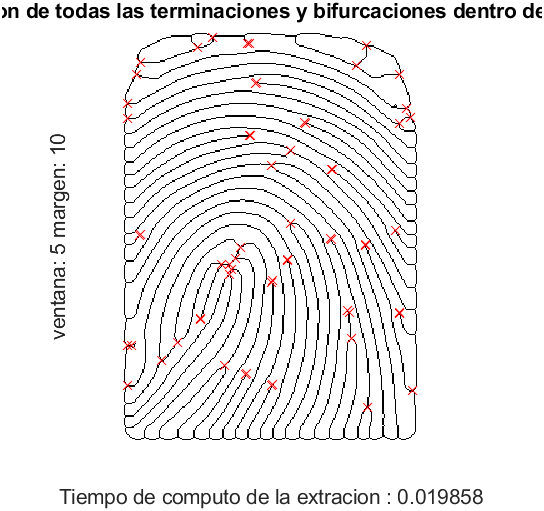
\includegraphics[scale=0.7]{Figures/Minutiae2-m10}
         \caption{Example1\_2}
     \end{subfigure}
    \caption{Minutiae of example fingerprints.}
    \label{fig:ex5b}
\end{figure}

As we can see, there are still some minutias found at the edge of the skeleton. Thus, there is still capability to increase the margin and still capture possible minutias situated at the edges. It is needed to make a \textbf{balance} between how many \emph{edge-minutias} you find and not ignoring any minutias that are close to the edges. \\

With this in mind, we decided to use a \textbf{margin of 13}, although other parameters in the range \(\{11,12,\dots,15\}\) could have been used as well.\\

Now, we try to \textbf{capture all the minutias} by reducing the window size. Since the initial window size is \(5\) and the window size must be \textbf{odd}, there is no other option than to use \(window = 3\).\\

With these considerations, we decided to use a \textbf{window size of 3}. The results obtained with the selected hyperparameters (window,margin) are the ones presented in Figure \ref{fig:ex5bfinal}.

\begin{figure}[H]
  \centering
       \begin{subfigure}[t]{0.45\textwidth}
         \centering
         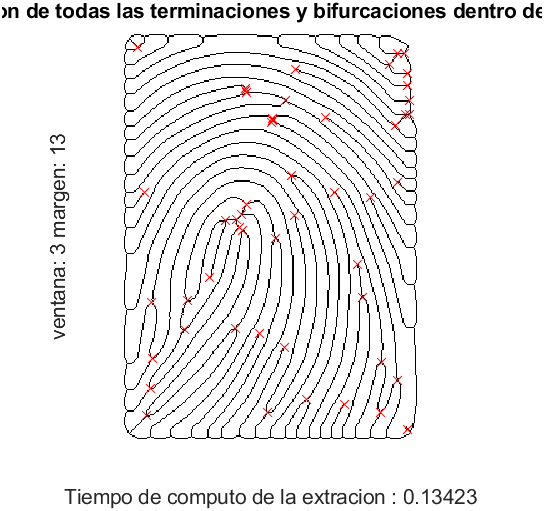
\includegraphics[scale=0.7]{Figures/Minutiae1-optim}
         \caption{Example1\_1}
     \end{subfigure}%
     \quad
     \begin{subfigure}[t]{0.45\textwidth}
         \centering
         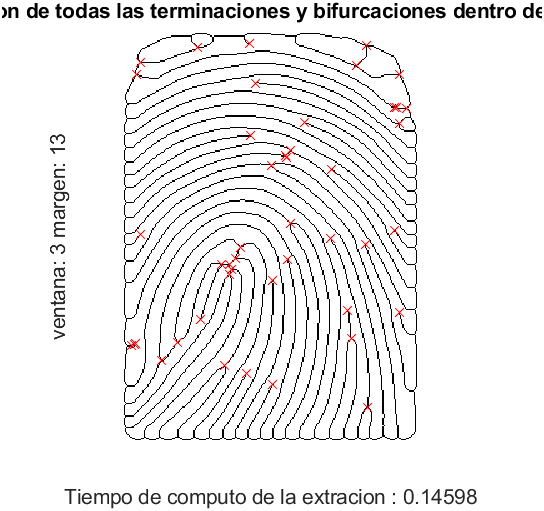
\includegraphics[scale=0.7]{Figures/Minutiae2-optim}
         \caption{Example1\_2}
     \end{subfigure}
    \caption{Minutiae extraction using optimal parameters: \(window = 3\), \(margin=13\).}
    \label{fig:ex5bfinal}
\end{figure}

As we can observe, all the minutias have been found (at least the ones that are easily visible) and there are not many minutias at/near the edges.


\section{Exercise 6}

\subsection{ Execute the code corresponding to the Minutiae Validation for window=5 and margin=5.  Paste the resulting image including the minutiae extracted (red crosses) and validated (blue circles) of both fingerprints. }

As we executed the code, we noticed that if we executed the given code, the images were printed complemented (black was white and vice-versa), so we added the following code to invert the images:
\begin{minted}{MatLab}
thin1_comp = imcomplement(thin1)
thin2_comp = imcomplement(thin2)
\end{minted}

Now, we show in Figure \ref{fig:ex6a} the result of the validation using the default parameters \(window = 5, margin = 5\).

\begin{figure}[H]
  \centering
       \begin{subfigure}[t]{0.45\textwidth}
         \centering
         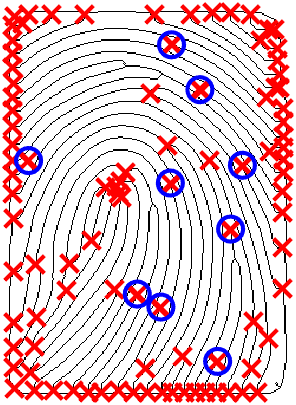
\includegraphics[scale=0.7]{Figures/Validation1-5-5}
         \caption{Example1\_1}
     \end{subfigure}%
     \quad
     \begin{subfigure}[t]{0.45\textwidth}
         \centering
         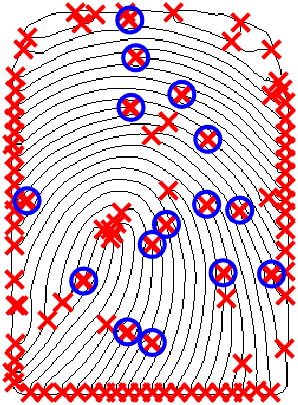
\includegraphics[scale=0.7]{Figures/Validation2-5-5}
         \caption{Example1\_2}
     \end{subfigure}
    \caption{Validation of minutiae extraction using parameters: \(window = 5\), \(margin=5\).}
    \label{fig:ex6a}
\end{figure}

As we can observe, many minutias have not been validated. The parameters that we have chosen in this case are not the optimal determined in the previous exercise.


\subsection{ Execute the same code but with the optimal values of parameters window and margin. Paste the resulting image below. }

The output obtained from the same code with the optimal values is the one presented in Figure \ref{fig:ex6b}.

\begin{figure}[H]
  \centering
       \begin{subfigure}[t]{0.45\textwidth}
         \centering
         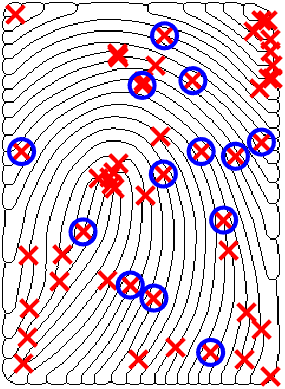
\includegraphics[scale=0.7]{Figures/Validation1-3-13}
         \caption{Example1\_1}
     \end{subfigure}%
     \quad
     \begin{subfigure}[t]{0.45\textwidth}
         \centering
         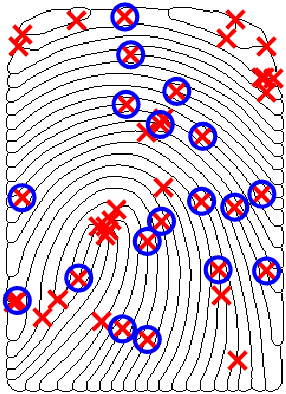
\includegraphics[scale=0.7]{Figures/Validation2-3-13}
         \caption{Example1\_2}
     \end{subfigure}
    \caption{Validation of minutias extraction using the optimal parameters.}
    \label{fig:ex6b}
\end{figure}

The result is similar to the previous one in terms of the validated minutias. There are a few more minutias validated in the case where the optimal \(window\) and \(margin\) are used.\\

As we did our experimentation with the parameters, we figured out that there is one more aspect that has to be taken into account: the \textbf{window size of the validation}. Until now, it was pre-set to one, but we can make it bigger to see what is the result.

\begin{figure}[H]
  \centering
       \begin{subfigure}[t]{0.45\textwidth}
         \centering
         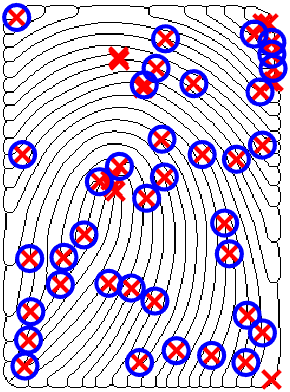
\includegraphics[scale=0.7]{Figures/Validation1-valwin7}
         \caption{Example1\_1}
     \end{subfigure}%
     \quad
     \begin{subfigure}[t]{0.45\textwidth}
         \centering
         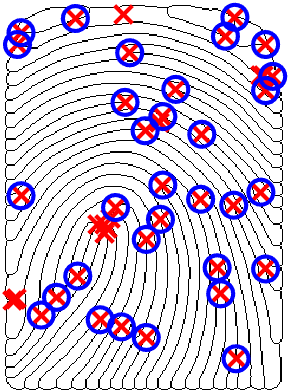
\includegraphics[scale=0.7]{Figures/Validation2-valwin7}
         \caption{Example1\_2}
     \end{subfigure}
    \caption{Validation of minutias extraction using optimal parameters and validation window size equal to \(7\).}
    \label{fig:ex6bval7}
\end{figure}

As we observe in Figure \ref{fig:ex6bval7}, when we increased the window size of the validation window, much more minutias were validated as we expected. This has its negative part too, since in a real problem it would have to be finetuned to obtain only the relevant minutias.  However, we will postulate that the more information about valid minutias, the better, so for the \textbf{optimal case}, we now use the parameter  \(validation\_window = 3\).


\subsection{ Do you think it is a good idea to include the Minutiae Validation module? Justify your opinion. }

In general, it \textbf{is good idea} to include the Minutiae Validation module, since sometimes all extracted minutias might not be relevant and we should be able to make a selection of the most important ones, which is performed in the validation selection. Furthermore, the extra window-size parameter in the validation stage all this preprocessing and extraction, gives us an extra degree of freedom in case we needed it for a Fingerprint detection problem.


\section{Extra Exercise}
With all the previous exercises done correctly you can obtain a mark up to 7 points out of 10. 
Extra work: If you want to obtain a mark up to 10 points out of 10 you should complete the following:
In folder “/ddbb” you have 20 fingerprint images. 19 of them are labeled with the subject identity (e.g., H0001), and 1 is Unknown. Search for the identity of the Unknown fingerprint in the set of 19 labelled reference fingerprints. You can use the provided code “identification\_1\_19.m” as basis. Paste here the resulting ranked list of scores of the Unknown fingerprint with respect each one of the 19 reference fingerprints.

\subsection{Solution}

The first thing that we will do is to complete the file \inline{extract_minutiae} in order to encapsulate all the useful code that we have done in \inline{main.m}. We will set the name of many variables to \inline{nil}, since they will be returned by the created functions but will not be used. The code of the created function is the following:

\begin{minted}{MatLab}
  function [valid_x,valid_y]=extract_minutiae(I,minutiae_window,minutiae_margin,val_window)

    % Enhance
    [nil, nil,nil,nil,relI,enhI] =  fft_enhance_cubs(I, -1);
    % Quality map
    [nil, binI, nil, nil, nil] =  testfin(enhI);  
    % Binarize and Segment Fingerprint
    threshold=0.9; 
    binI(relI<threshold)=0; 
    inv_binI = (binI == 0);
    %Fingerprint Skeleton
    thin =  bwmorph(inv_binI, 'thin',Inf);

    %Minutiae Extractor          
    [minutiae, minutiae_x, minutiae_y,nil]=extraction(thin,minutiae_window,minutiae_margin);

    %Minutiae Validation
    [nil, valid_x, valid_y, nil]=validation(thin,minutiae,val_window);

end
\end{minted}

Using this code, in this exercise we only have to extract minutias for each of the candidates and compare them with the unlabeled fingerprints to detect which one has the highest coincidence. The code that performs this action is too long to be included in this memory, so it is attached as a file: \inline{identification_1_19.m}.

Until this point, we have made several choices in the parameters \(window,margin\) and  \(validation\_window\). In this last exercise, we test with a few possible combinations of those, to check if our previous decissions help in this problem.

\subsubsection{Initially proposed parameters}

Firstly, we test the \textbf{first parameters} that were proposed, which are \(window = 5, margin = 5,validation\_margin = 1\) (we have selected this validation margin )

\begin{table}[H]
  \centering
  \begin{tabular}{lrrrrrrrrrr}

    {} &    1  &    2  &    3  &    4  &    5  &    6  &    7  &    8  &    9  &    10 \\
    \midrule
    Hough &  0.21 &  0.16 &  0.18 &  0.16 &  0.12 &  0.12 &  0.17 &  0.22 &  0.16 &  0.17 \\

    \end{tabular}
    
    \begin{tabular}{lrrrrrrrrr}

    {} &    11 &    12 &    13 &   14 &    15 &    16 &    17 &    18 &    19 \\
    \midrule
     &  0.12 &  0.18 &  \textbf{0.53} &  0.2 &  0.16 &  0.18 &  0.19 &  0.12 &  0.18 \\

    \end{tabular}
    
    \caption{Results for the initial parameters.}

\end{table}


As we can see, the selected subject is the \textbf{number thirteen}, with a coincidence of \(53\%\), doubling the score of all the rest of the prints.

\subsection{Optimal parameters with small validation window}

We decided to firsly test the \textbf{optimal parameters} (which are \(window = 3, margin = 13\) ) with a validation window size of \(1\). The results are the following:

\begin{table}[H]
  \centering
  \begin{tabular}{lrrrrrrrrrr}

    {} &    1  &    2  &   3  &    4  &    5  &    6  &    7  &    8  &    9  &    10 \\
    \midrule
    Hough &  0.19 &  0.15 &  0.2 &  0.15 &  0.12 &  0.14 &  0.17 &  0.23 &  0.18 &  0.18 \\

    \end{tabular}
    
    \begin{tabular}{lrrrrrrrrr}

    {} &    11 &   12 &    13 &   14 &    15 &   16 &   17 &    18 &   19 \\
    \midrule
     &  0.12 &  0.2 &  \textbf{0.55} &  0.2 &  0.16 &  0.2 &  0.2 &  0.13 &  0.2 \\

    \end{tabular}
    
    \caption{Results for the optimal parameters and validation window equal to \(1\).}

\end{table}

As we can see, using the optimal parameters gives us a little improvement in the percentage of coincidence using Hough in the correct case, and the rest of the cases vary: some increase its percentage of coincidence (by no more than \(2\%\)) and some of them decrease this Hough coefficient. However, it may be happening what we saw when we used no validation: there could be many minutias that are not very relevant that are coincident in all the fingerprints.\\

We still postulate that the unknown fingerprint belongs to subject 13.


\subsubsection{Optimal parameters with bigger validation window}

Now, we test the postulated \textbf{optimal parameters}, which are \(window = 3, margin = 13,validation\_margin = 3\) 

\begin{table}[H]
  \centering
  \begin{tabular}{lrrrrrrrrrr}

    {} &    1  &    2  &   3  &    4  &    5  &    6  &    7  &    8  &    9  &    10 \\
    \midrule
    Hough &  0.25 &  0.23 &  0.3 &  0.23 &  0.19 &  0.18 &  0.22 &  0.26 &  0.23 &  0.19 \\

    \end{tabular}
    
    \begin{tabular}{lrrrrrrrrr}

    {} &   11 &    12 &    13 &    14 &   15 &    16 &    17 &    18 &    19 \\
    \midrule
     &  0.2 &  0.26 &  \textbf{0.67} &  0.24 &  0.2 &  0.23 &  0.24 &  0.18 &  0.24 \\

    \end{tabular}
  \caption{Results for the optimal parameters.}
\end{table}


This case increases the Hough scores in all cases, but really highlights a case: the number thirteen. We confirm in this case that the optimal parameters are providing us with good quality information about the suspects, increasing the percentage of coincidence.

\subsubsection{Checking smaller margin}

In a previous exercise, we chose a margin of \(13\) since using it removed many minutias from the edges that we believed to be probably not useful. We now check if reducing this margin to a middle point between the initial  (\(5\)) and the chosen as optimal (\(13\)) turns into higher coincidence with the subjects or not. We execute the identifiation code with parameters \(window = 3, margin = 8, val\_window = 3 \) and obtain the following results.

\begin{table}[H]
  \centering
  \begin{tabular}{lrrrrrrrrrr}

    {} &    1  &    2  &    3  &    4  &    5  &    6  &    7  &    8  &    9  &    10 \\
    \midrule
    Hough &  0.32 &  0.27 &  0.29 &  0.28 &  0.27 &  0.28 &  0.29 &  0.29 &  0.31 &  0.26 \\

    \end{tabular}
    
    \begin{tabular}{lrrrrrrrrr}

    {} &    11 &    12 &    13 &    14 &    15 &    16 &    17 &    18 &    19 \\
    \midrule
     &  0.27 &  0.29 &  \textbf{0.79} &  0.33 &  0.29 &  0.26 &  0.29 &  0.27 &  0.28 \\

    \end{tabular}
  \caption{Results using middlepoint window.}
\end{table}

Again, we obtained that the subject with more coincidence is the \textbf{number 13}.

\subsubsection{Conclusions}

With all this cases tested, we can confirm with a high grade of confidence that the unknown fingerprint corresponds to \textbf{suspect 13}.\\

It has to be mentioned that as we can see in Figure \ref{fig:extra:comparison} the hyperparameters:
\[
window = 3, \quad margin = 8, \quad val\_window = 3  
\]
were the ones that resulted in higher coincidence in our number 13 candidate.

\begin{figure}[H]
\centering
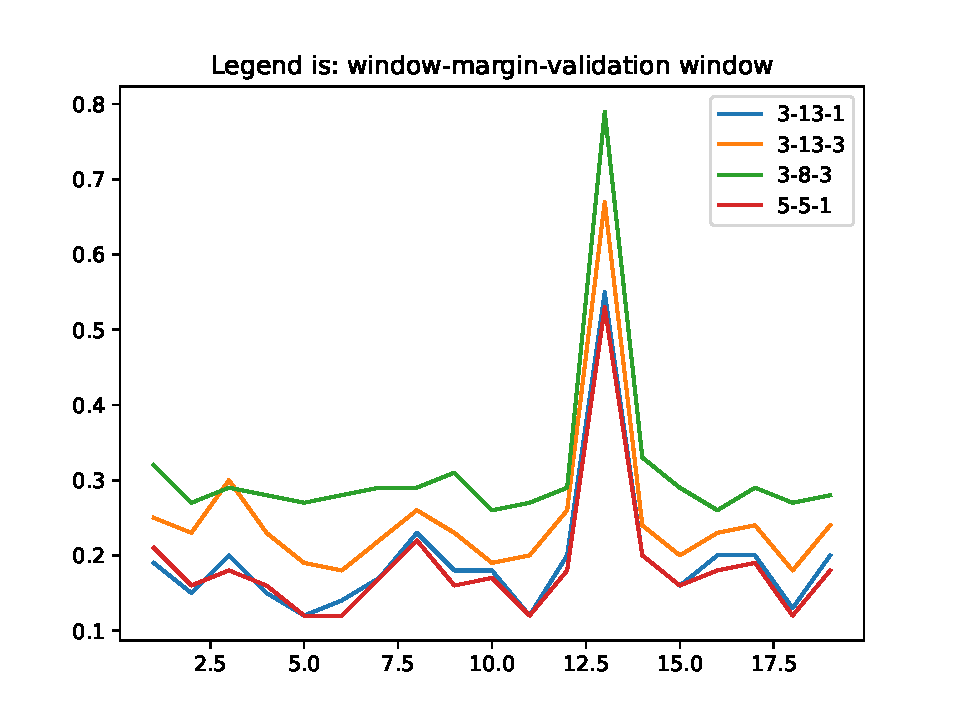
\includegraphics[scale=0.8]{Results}
\caption{Comparison of Hough coefficients for the different hyperparameter configurations.}
\label{fig:extra:comparison}
\end{figure}

However, as we can see, when a set of parameters increases the coincidence percentage with our main subject, it \emph{proportionally} does the same for all the subjects. In this case, is not very relevant since it is clear that the coincidence percentage is \textbf{quite higher} for subject number 13. However, in other identification problems where the coincidences between the fingerprints or the minutias of the subjects are more similar, the set of parameters should be selected carefully.

\end{document}